\chapter{Competing order during heterogeneous nucleation}
\label{ch:crystallisation}

\section{Crystallisation at the wall}

It is well known that a flat wall induces layering in a fluid~\citep{Barrat1999, Mugele2000, Brovchenko2005, Dammer2006}. In a gas, this can induce capillary condensation of the liquid. In a  dense liquid, this layering effect often lead to heterogeneous crystallisation~\citep{Gelb1999, Kegel2001}. In our colloidal suspensions, we observed frequently density oscillations near the wall over the distance of $5\sim10\sigma$. Despite the polydispersity of our particles, the first few crystalline layers are obviously crystalline and sometime a crystal grows from the wall and invades the bulk.

The initial layering occurs parallel to the wall and orients in the same way the hexatic planes. However the growth speed is very heterogeneous, leading to a complicated landscape of crystalline mountains and fluid valleys, as displayed in \FigureRef{fig:X_mountains}.

\begin{figure}
	\centering
	\begin{small}%
	\tikz\shade[ball color=red!80!white] circle (0.4em);
	Crystal\qquad%
	\tikz\shade[ball color=white] circle (0.4em);
	Two first layers\qquad%
	\tikz\shade[ball color=blue] circle (0.4em);
	\acs{FCC}\qquad%
	\tikz\shade[ball color=yellow] circle (0.4em);
	\acs{HCP}%
	\end{small}\\
	\subfloat[Coloured by $Q_6$. Red is high values.]{
		\label{fig:X_mountains_Q6}
		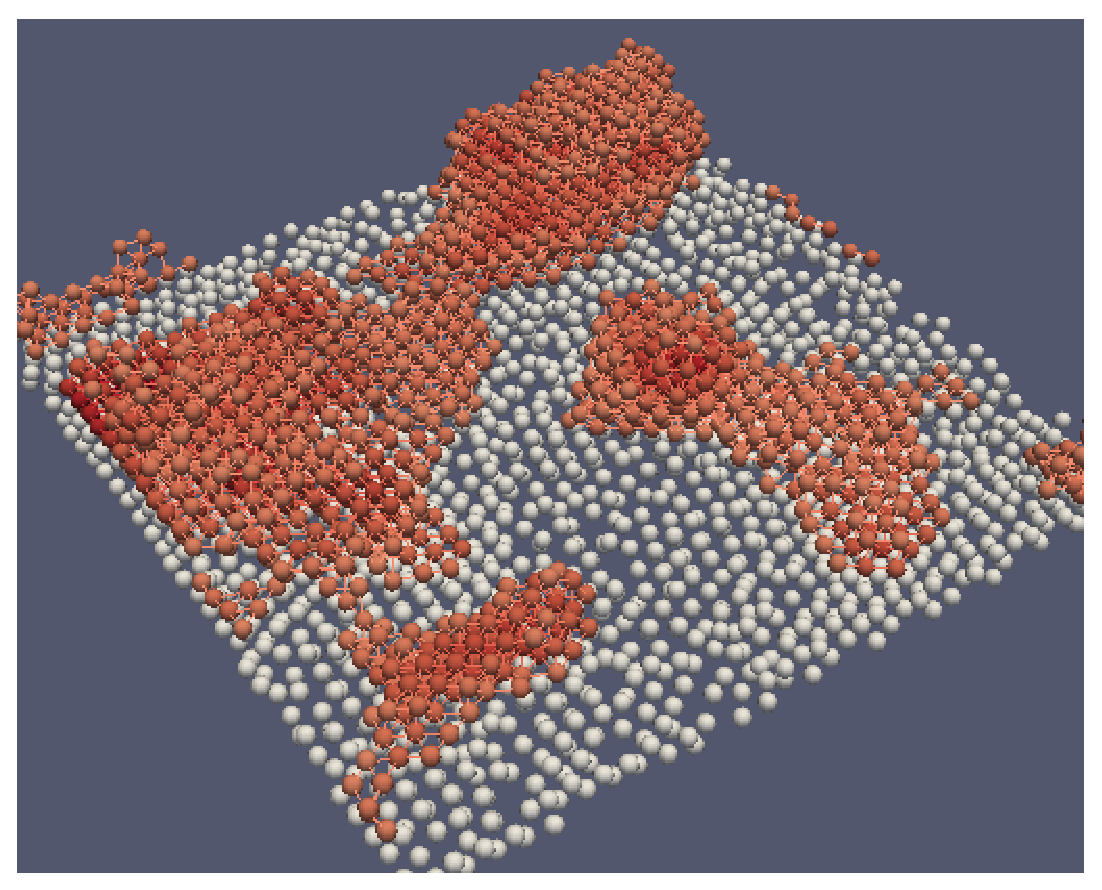
\includegraphics[width=0.45\textwidth]{X_mountains_Q6}}\quad
	\subfloat[Coloured by $W_4$. Blue is negative (\acs{FCC}) and yellow positive (\acs{HCP})]{
		\label{fig:X_mountains_W4}
		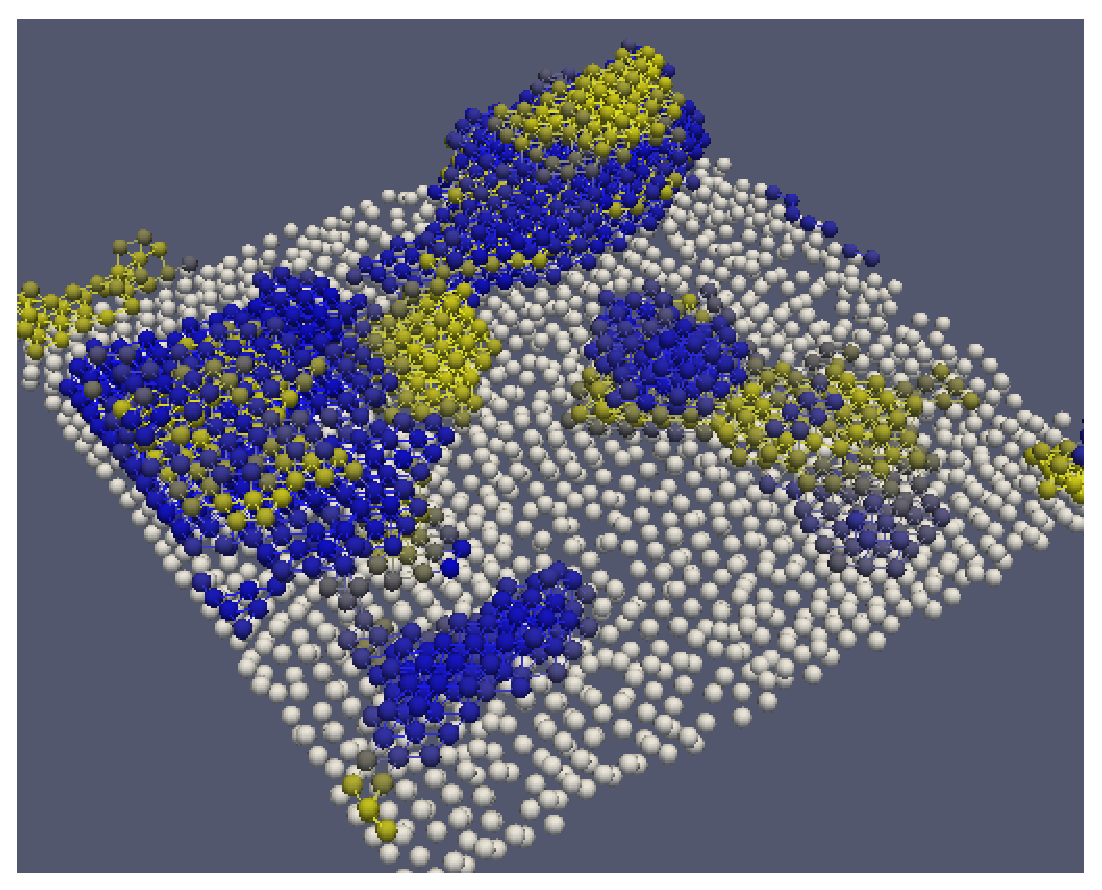
\includegraphics[width=0.45\textwidth]{X_mountains_W4}}
	\caption{Views of crystals nucleated from wall. Are shown only the particles with $Q_6>0.4$ and the two first layers (in white) that could not be analysed by coarse-grained \acs{BOO}.}
	\label{fig:X_mountains}
\end{figure}

According to \citet{Kawasaki2010} the homogeneous nucleation of crystals in hard spheres is linked to the fluctuations of the crystal-like bond order parameter $Q_6$. Crystals nucleate in regions of high $Q_6$. However, the link between bond order fluctuations and \emph{heterogeneous} nucleation has not yet been investigated.

To start from a well-defined state, we prepare a supercooled sample at the density-matching temperature. This takes some time during which crystallites have already formed at the wall. Then, we heat up our sample by a few degrees compared to the density-matching temperature in order to make the colloids heavier than the solvent. The volume fraction at the top of the sample (close to the objective lens and thus allowing much clear imaging) drops, so that this part of the sample is not supercooled. We confirm that all crystallites and crystal-like bond order have disappeared from the region of the wall. Finally, we set back the thermostat to the density-matching temperature, allowing the top of the sample to slowly return to its supercooled state. We could then observe the heterogeneous nucleation from the beginning. We tracked the sample from top to bottom and we are thus sure that the crystallite actually form at the wall and do not come from the rest of the sample.

\begin{figure}
	\centering
	\begin{small}%
	\tikz\shade[ball color=green!33!black] circle (0.4em);
	Crystal-like\qquad%
	\tikz\shade[ball color=red!80!black] circle (0.4em);
	Crystal\qquad%
	\tikz\shade[ball color=white] circle (0.4em);
	Two first layers%
	\end{small}\\
	\subfloat[$t=0$]{\label{fig:X_t000}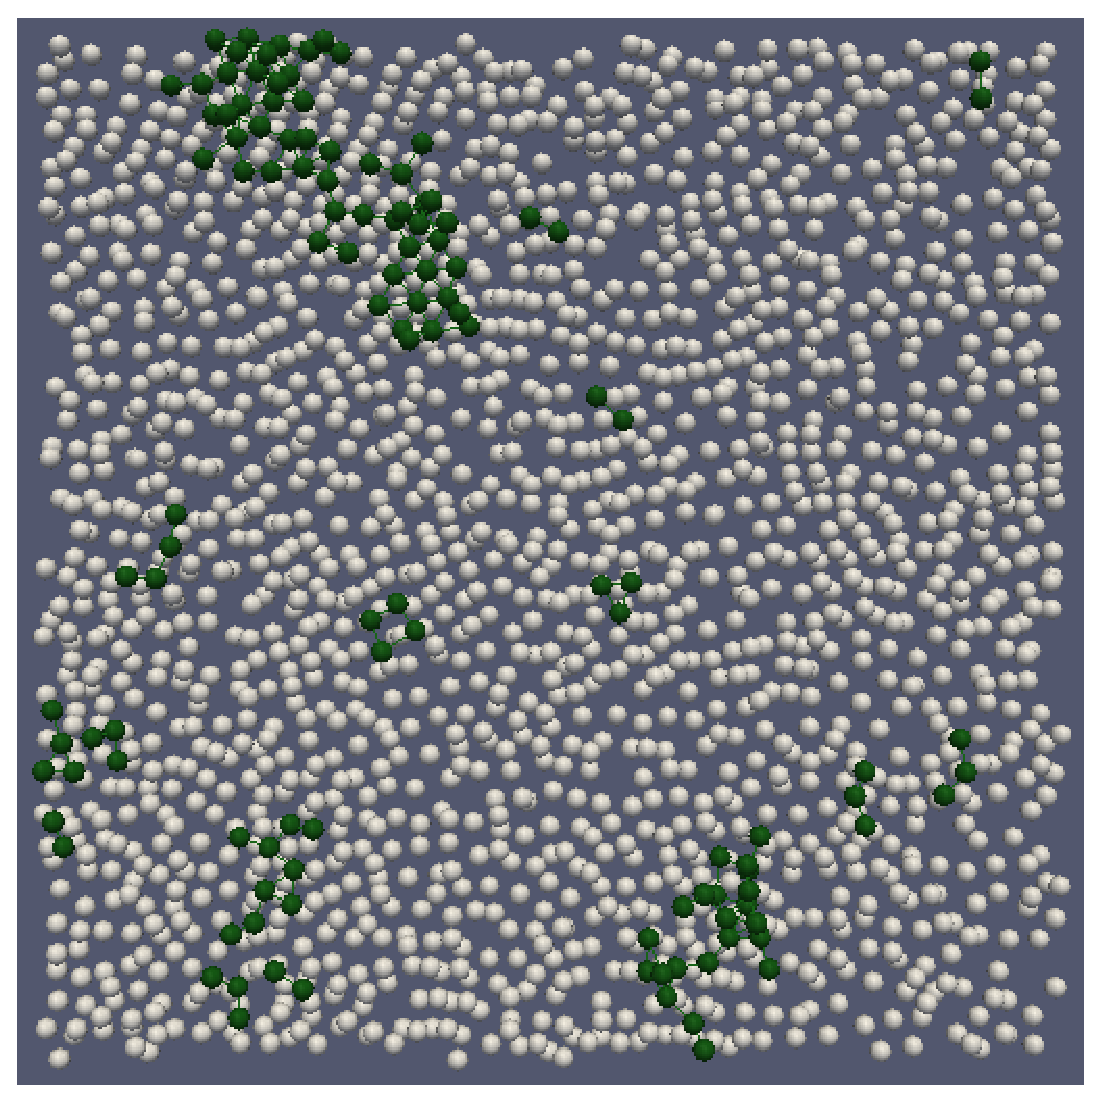
\includegraphics[width=0.25\textwidth]{X_t000}}
	\subfloat[$t=\unit{5}{\hour}$]{\label{fig:X_t025}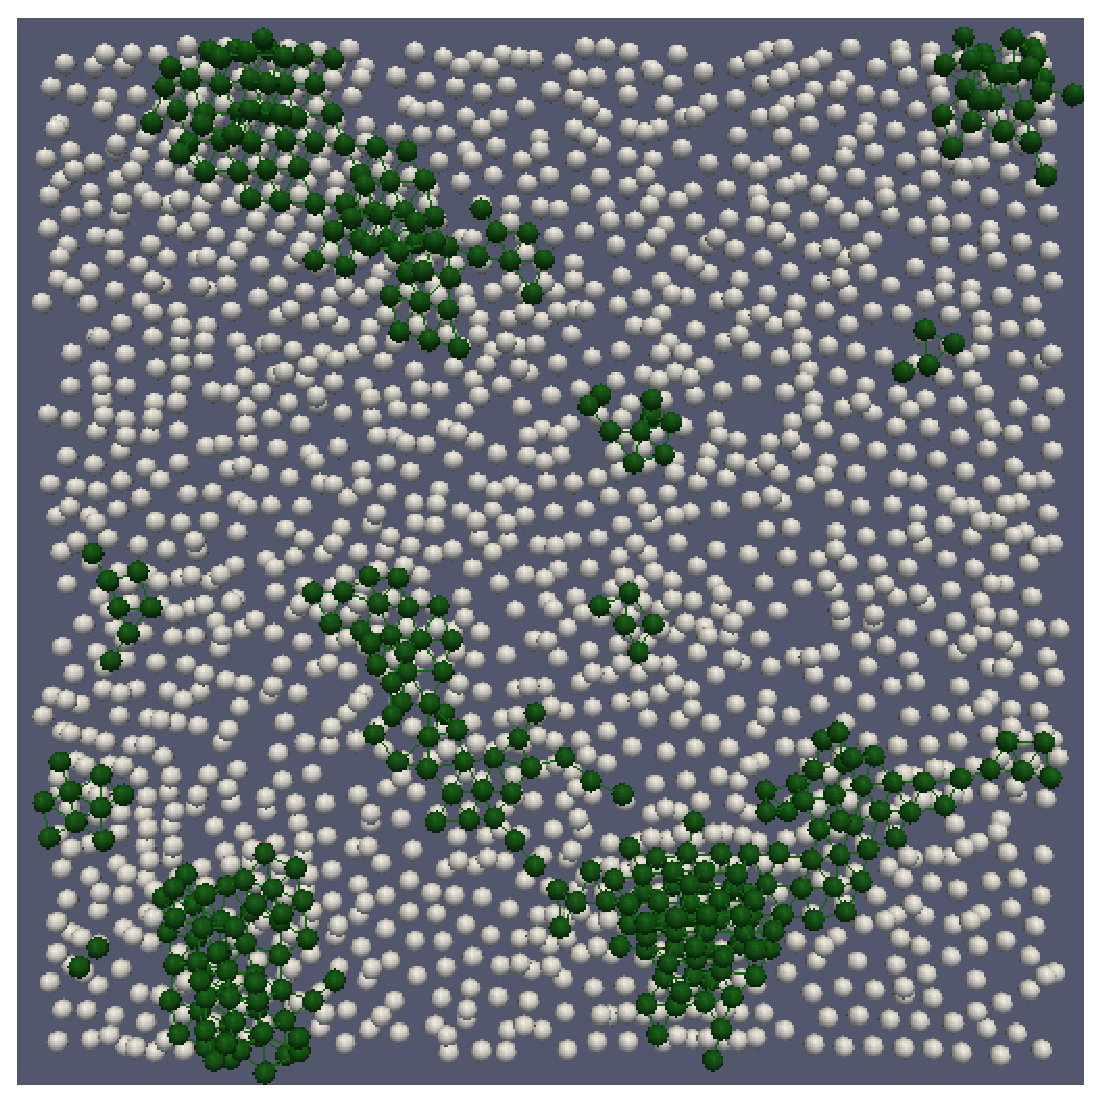
\includegraphics[width=0.25\textwidth]{X_t025}}
	\subfloat[$t=\unit{10}{\hour}$]{\label{fig:X_t050}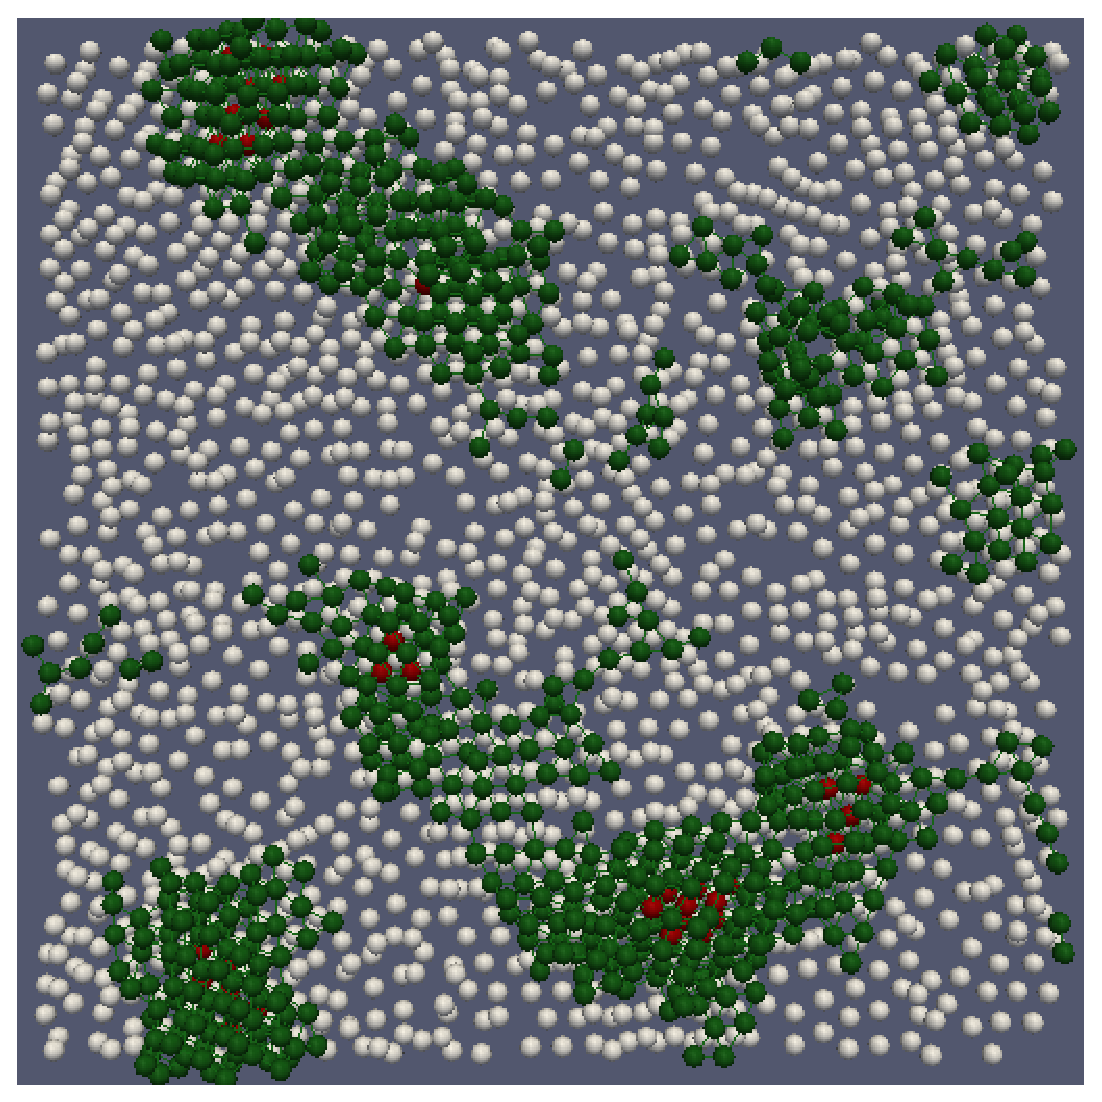
\includegraphics[width=0.25\textwidth]{X_t050}}
	\subfloat[$t=\unit{15}{\hour}$]{\label{fig:X_t075}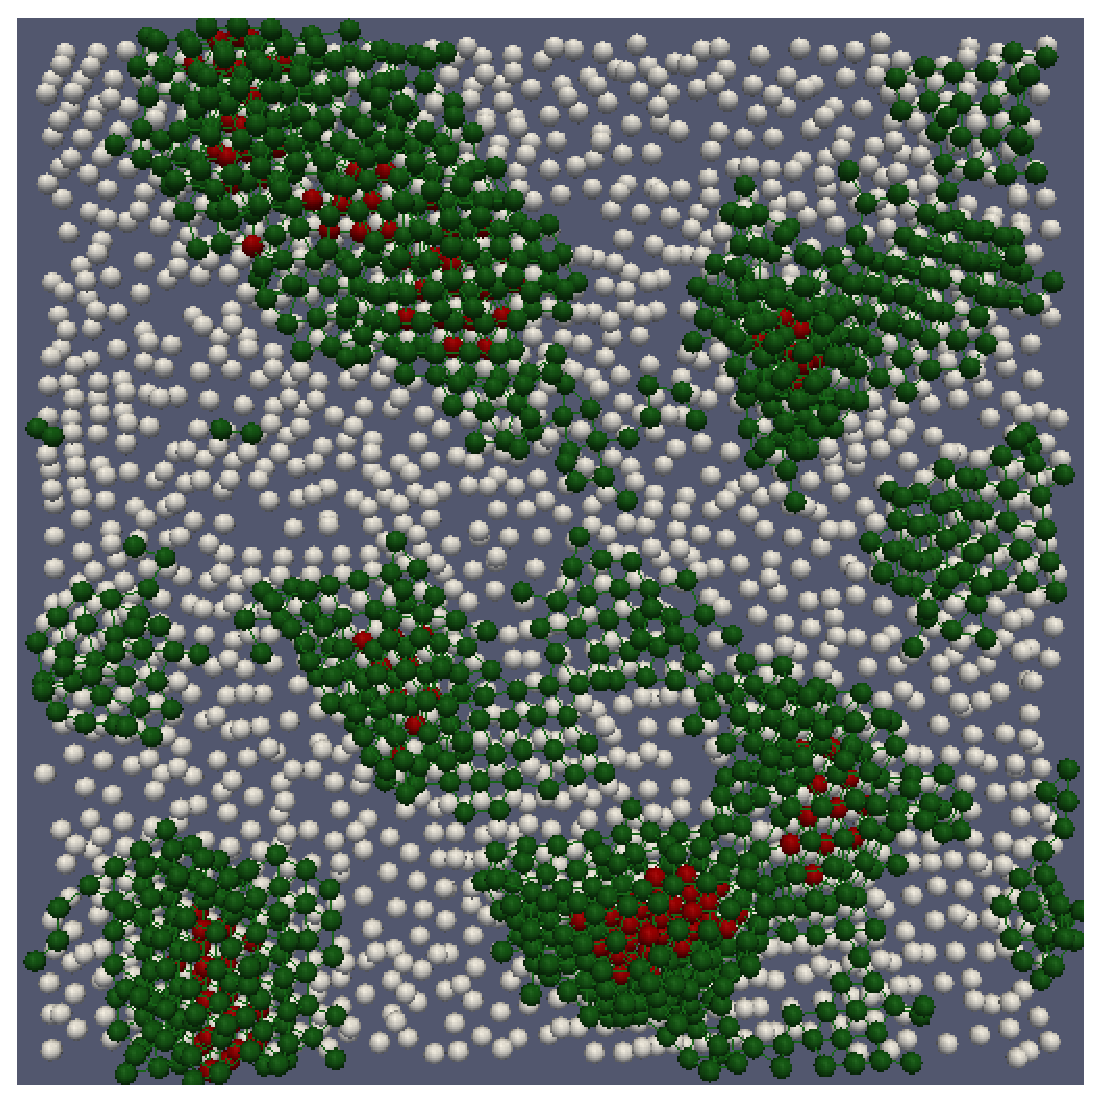
\includegraphics[width=0.25\textwidth]{X_t075}}\\
	\subfloat[$t=\unit{20}{\hour}$]{\label{fig:X_t100}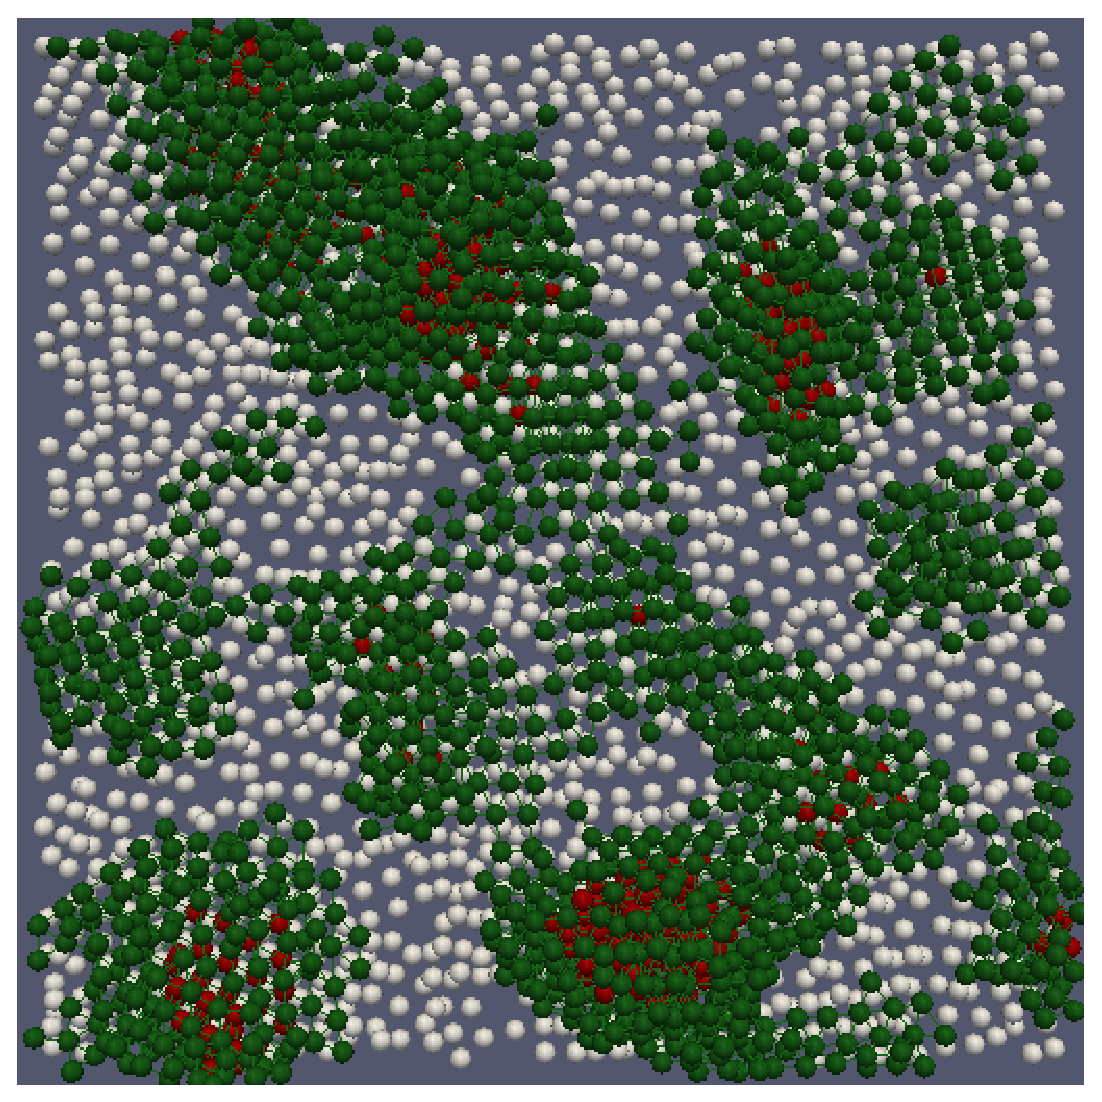
\includegraphics[width=0.25\textwidth]{X_t100}}
	\subfloat[$t=\unit{30}{\hour}$]{\label{fig:X_t150}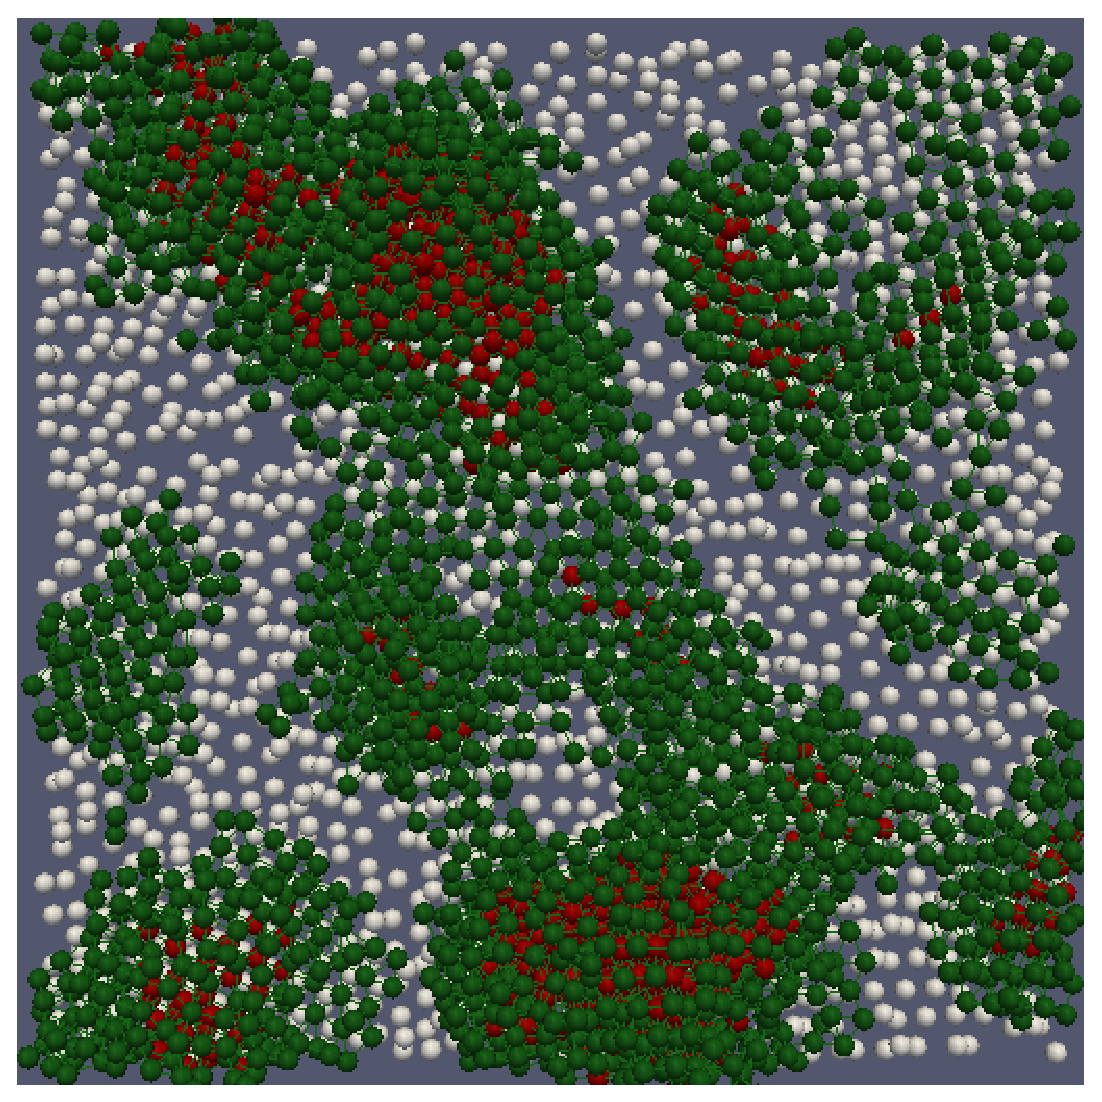
\includegraphics[width=0.25\textwidth]{X_t150}}
	\subfloat[$t=\unit{40}{\hour}$]{\label{fig:X_t200}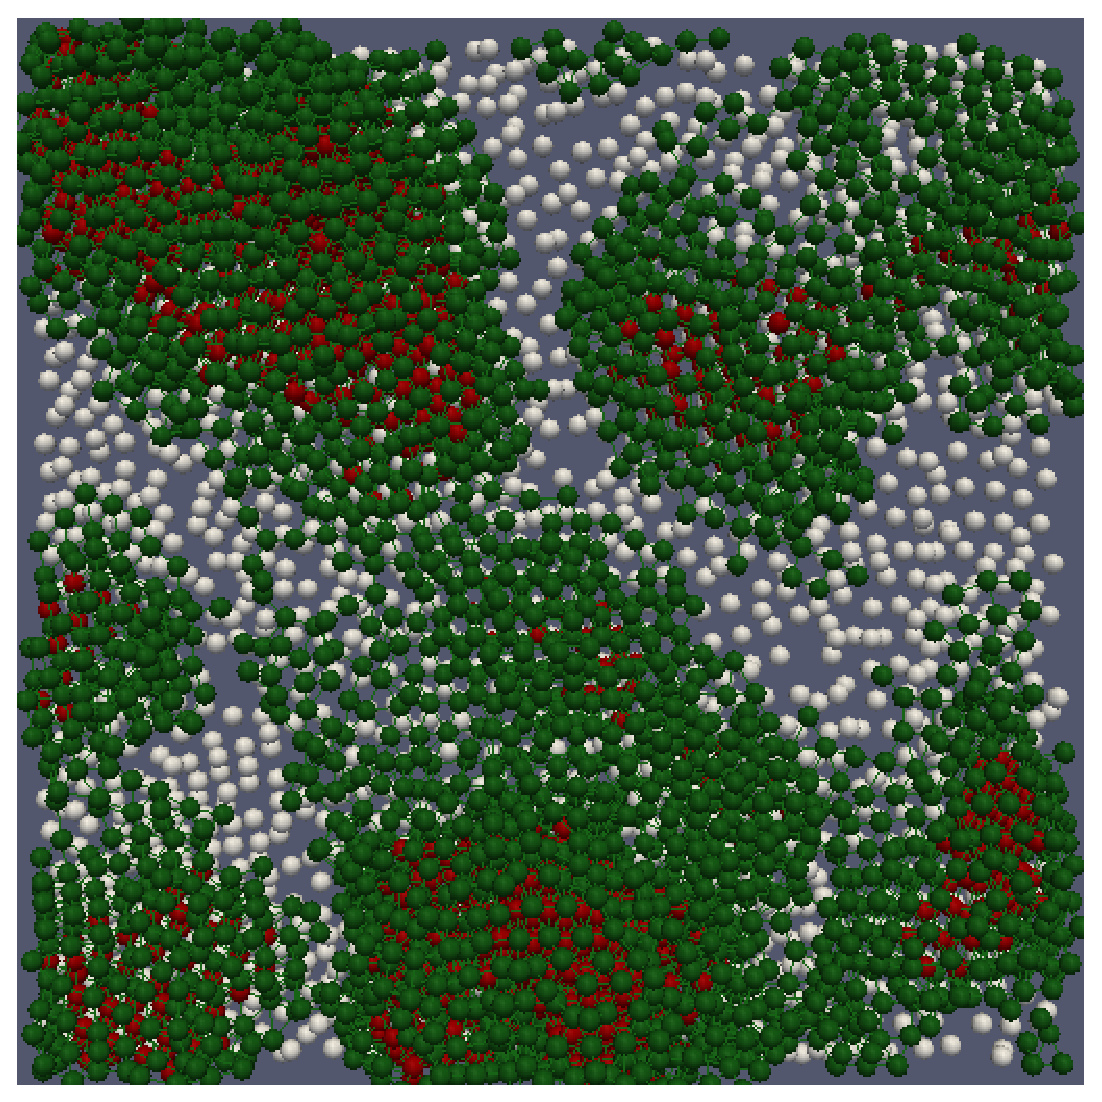
\includegraphics[width=0.25\textwidth]{X_t200}}
	\subfloat[$t=\unit{60}{\hour}$]{\label{fig:X_t299}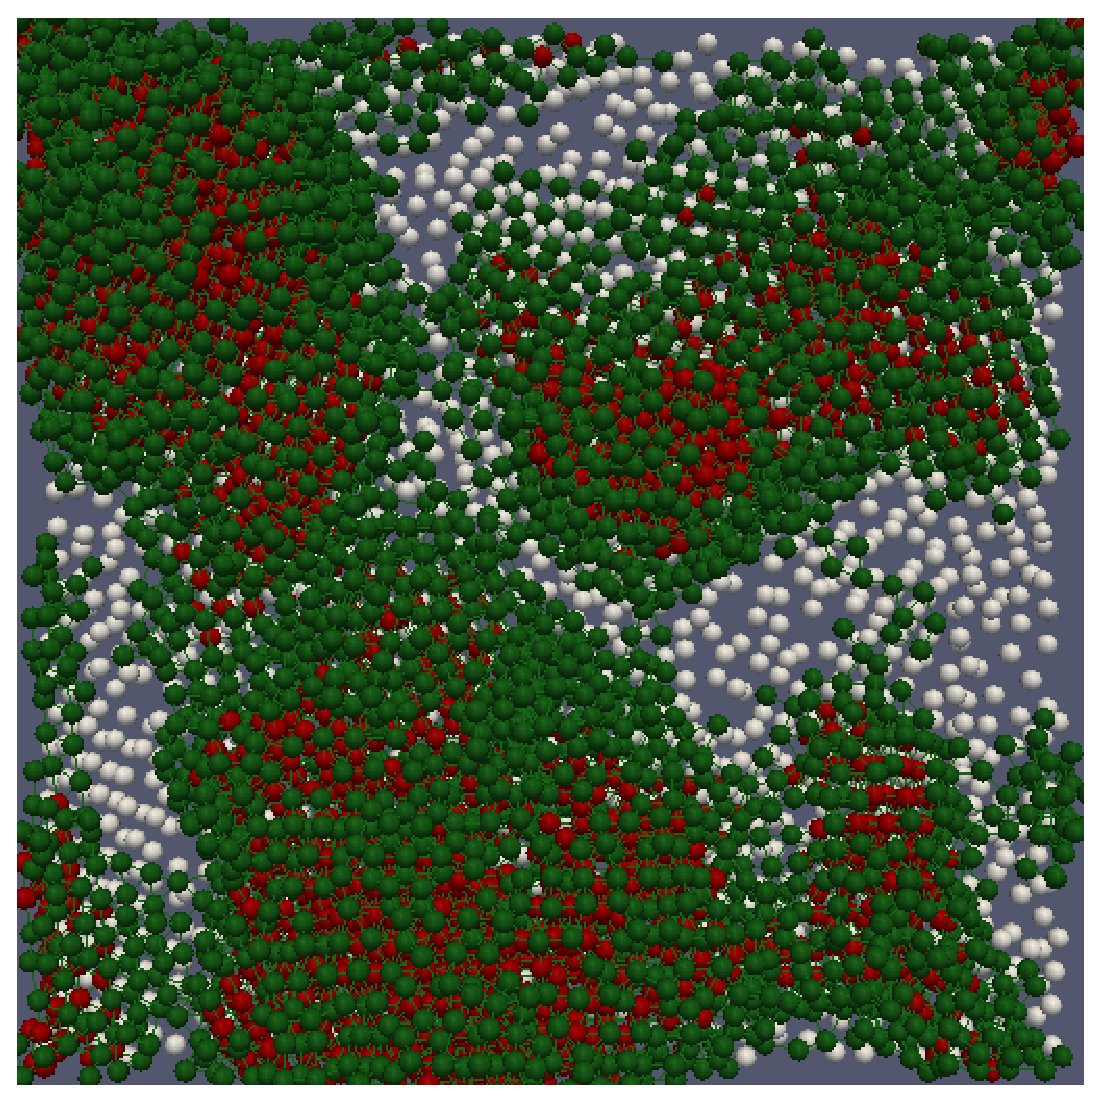
\includegraphics[width=0.25\textwidth]{X_t299}}
	\caption{Heterogeneous crystal nucleation and growth. (green) The crystal-like bond ordered particles with $0.25<Q_6<0.4$; (red) the crystals $0.4<Q_6$; (white) the two first layers that could not be analysed by coarse-grained \acs{BOO}.}
	\label{fig:X_growth}
\end{figure}

Snapshots of the growth are presented in \FigureRef{fig:X_growth}. We see clearly that the crystal nucleus originate from the fluctuations of the crystalline bond order at the surface. Then, rather than starting newly from different parts of the wall, the bond order covers the already formed nuclei and thus the crystal grows. This explains the heterogeneities in crystalline growth speed.

It is easier to form a hexatic plane against a wall than in contact with a disordered environment of particles. In some sense, the crystal-like bond order has an affinity for the flat wall. However, the affinity is even stronger for an already formed crystal. So the crystal grows rather than covering the surface of the wall. Everything appends as in a partial wetting phenomenon, except that we have no attraction to explain the wetting.

\section{Role of the icosahedral order}

The heterogenenous nucleation is also an occasion to study the relationship between the crystal-like bond order and the icosahedral bond order. We know that geometrically they are mutually exclusive, but we do not know how long ranged is this exclusion.

\begin{figure}
	\centering
	\resizebox{\textwidth}{!}{\input{X_profile}}
	\caption{Number density profile (arbitrary scale) along depth $z$ of: all the particles, the crystal-like bond ordered particles ($Q_6>0.25$), the icosahedral particles ($w6<w_6^{dodec}$) and the crystal particles ($Q_6>0.4$).}
	\label{fig:X_profile}
\end{figure}

In \FigureRef{fig:X_profile}, we plotted the evolution of the density profiles of the different structures during the heterogeneous nucleation and growth. We first notice that the density oscillations always extend $\simeq 2\sigma$ further from the wall compared to the front of crystal-like bond ordered particles. This means that in the case of heterogeneous nucleation the layering appends first, and then the bond ordering.

We notice then that the number density of the icosahedral particles is also oscillating in phase with the total number density and the \ac{MRCO} number density. Even a structure without periodicity is affected by the layering. However, $\rho_{ico}$ falls when entering the crystal-like ordered region. We have two possible hypothesis to explain this phenomenon:
\begin{enumerate}
	\item\label{hyp:disruption} The icosahedral structure is disrupted by the crystalline order growth or the layering.
	\item\label{hyp:excluded_vol} The icosahedral structure cannot penetrate inside the crystal-like order but is not disrupted by the layering and can penetrate in the valleys between the crystals.
\end{enumerate}
To decide between these hypotheses, we plot in \FigureRef{fig:X_profile_normed} the number density of icosahedra considering only the volume outside of the \ac{MRCO}:
\begin{equation}
\rho_{ico}^* \equiv \rho_{ico}/(\rho-\rho_{mrco})
\end{equation}

\begin{figure}
	\centering
	\resizebox{\textwidth}{!}{% GNUPLOT: LaTeX picture with Postscript
\begingroup
  \makeatletter
  \providecommand\color[2][]{%
    \GenericError{(gnuplot) \space\space\space\@spaces}{%
      Package color not loaded in conjunction with
      terminal option `colourtext'%
    }{See the gnuplot documentation for explanation.%
    }{Either use 'blacktext' in gnuplot or load the package
      color.sty in LaTeX.}%
    \renewcommand\color[2][]{}%
  }%
  \providecommand\includegraphics[2][]{%
    \GenericError{(gnuplot) \space\space\space\@spaces}{%
      Package graphicx or graphics not loaded%
    }{See the gnuplot documentation for explanation.%
    }{The gnuplot epslatex terminal needs graphicx.sty or graphics.sty.}%
    \renewcommand\includegraphics[2][]{}%
  }%
  \providecommand\rotatebox[2]{#2}%
  \@ifundefined{ifGPcolor}{%
    \newif\ifGPcolor
    \GPcolortrue
  }{}%
  \@ifundefined{ifGPblacktext}{%
    \newif\ifGPblacktext
    \GPblacktexttrue
  }{}%
  % define a \g@addto@macro without @ in the name:
  \let\gplgaddtomacro\g@addto@macro
  % define empty templates for all commands taking text:
  \gdef\gplbacktext{}%
  \gdef\gplfronttext{}%
  \makeatother
  \ifGPblacktext
    % no textcolor at all
    \def\colorrgb#1{}%
    \def\colorgray#1{}%
  \else
    % gray or color?
    \ifGPcolor
      \def\colorrgb#1{\color[rgb]{#1}}%
      \def\colorgray#1{\color[gray]{#1}}%
      \expandafter\def\csname LTw\endcsname{\color{white}}%
      \expandafter\def\csname LTb\endcsname{\color{black}}%
      \expandafter\def\csname LTa\endcsname{\color{black}}%
      \expandafter\def\csname LT0\endcsname{\color[rgb]{1,0,0}}%
      \expandafter\def\csname LT1\endcsname{\color[rgb]{0,1,0}}%
      \expandafter\def\csname LT2\endcsname{\color[rgb]{0,0,1}}%
      \expandafter\def\csname LT3\endcsname{\color[rgb]{1,0,1}}%
      \expandafter\def\csname LT4\endcsname{\color[rgb]{0,1,1}}%
      \expandafter\def\csname LT5\endcsname{\color[rgb]{1,1,0}}%
      \expandafter\def\csname LT6\endcsname{\color[rgb]{0,0,0}}%
      \expandafter\def\csname LT7\endcsname{\color[rgb]{1,0.3,0}}%
      \expandafter\def\csname LT8\endcsname{\color[rgb]{0.5,0.5,0.5}}%
    \else
      % gray
      \def\colorrgb#1{\color{black}}%
      \def\colorgray#1{\color[gray]{#1}}%
      \expandafter\def\csname LTw\endcsname{\color{white}}%
      \expandafter\def\csname LTb\endcsname{\color{black}}%
      \expandafter\def\csname LTa\endcsname{\color{black}}%
      \expandafter\def\csname LT0\endcsname{\color{black}}%
      \expandafter\def\csname LT1\endcsname{\color{black}}%
      \expandafter\def\csname LT2\endcsname{\color{black}}%
      \expandafter\def\csname LT3\endcsname{\color{black}}%
      \expandafter\def\csname LT4\endcsname{\color{black}}%
      \expandafter\def\csname LT5\endcsname{\color{black}}%
      \expandafter\def\csname LT6\endcsname{\color{black}}%
      \expandafter\def\csname LT7\endcsname{\color{black}}%
      \expandafter\def\csname LT8\endcsname{\color{black}}%
    \fi
  \fi
  \setlength{\unitlength}{0.0500bp}%
  \begin{picture}(7200.00,5040.00)%
    \gplgaddtomacro\gplbacktext{%
      \csname LTb\endcsname%
      \put(924,704){\makebox(0,0)[r]{\strut{}$0$}}%
      \put(924,1259){\makebox(0,0)[r]{\strut{}$0.2$}}%
      \put(924,1813){\makebox(0,0)[r]{\strut{}$0.4$}}%
      \put(924,2368){\makebox(0,0)[r]{\strut{}$0.6$}}%
      \put(924,2922){\makebox(0,0)[r]{\strut{}$0.8$}}%
      \put(924,3477){\makebox(0,0)[r]{\strut{}$1$}}%
      \put(924,4031){\makebox(0,0)[r]{\strut{}$1.2$}}%
      \put(1056,484){\makebox(0,0){\strut{}$2$}}%
      \put(1934,484){\makebox(0,0){\strut{}$4$}}%
      \put(2811,484){\makebox(0,0){\strut{}$6$}}%
      \put(3689,484){\makebox(0,0){\strut{}$8$}}%
      \put(4566,484){\makebox(0,0){\strut{}$10$}}%
      \put(5444,484){\makebox(0,0){\strut{}$12$}}%
      \put(6321,484){\makebox(0,0){\strut{}$14$}}%
      \put(286,2367){\rotatebox{90}{\makebox(0,0){\strut{}Number density}}}%
      \put(6979,2367){\rotatebox{90}{\makebox(0,0){\strut{}}}}%
      \put(3908,154){\makebox(0,0){\strut{}$z/\sigma$}}%
      \put(3908,3921){\makebox(0,0){\strut{}}}%
      \put(3908,3920){\makebox(0,0){\strut{}}}%
      \put(132,110){\makebox(0,0)[l]{\strut{}}}%
      \put(3908,3366){\makebox(0,0){\strut{}$t=\unit{40}{\hour}$}}%
    }%
    \gplgaddtomacro\gplfronttext{%
      \csname LTb\endcsname%
      \put(5773,2697){\makebox(0,0)[r]{\strut{}$\rho_{mrco}/\rho$}}%
      \csname LTb\endcsname%
      \put(5773,2367){\makebox(0,0)[r]{\strut{}$\rho_{ico}/\rho$}}%
      \csname LTb\endcsname%
      \put(5773,2037){\makebox(0,0)[r]{\strut{}$\rho_{ico}/(\rho-\rho_{mrco})$}}%
    }%
    \gplgaddtomacro\gplbacktext{%
      \csname LTb\endcsname%
      \put(924,4294){\makebox(0,0)[r]{\strut{}$0.1$}}%
      \put(924,4557){\makebox(0,0)[r]{\strut{}$0.2$}}%
      \put(924,4819){\makebox(0,0)[r]{\strut{}$0.3$}}%
      \put(1056,3812){\makebox(0,0){\strut{}}}%
      \put(1934,3812){\makebox(0,0){\strut{}}}%
      \put(2811,3812){\makebox(0,0){\strut{}}}%
      \put(3689,3812){\makebox(0,0){\strut{}}}%
      \put(4566,3812){\makebox(0,0){\strut{}}}%
      \put(5444,3812){\makebox(0,0){\strut{}}}%
      \put(6321,3812){\makebox(0,0){\strut{}}}%
      \put(6979,4425){\rotatebox{90}{\makebox(0,0){\strut{}}}}%
      \put(3908,4709){\makebox(0,0){\strut{}}}%
      \put(3908,4708){\makebox(0,0){\strut{}}}%
      \put(132,3922){\makebox(0,0)[l]{\strut{}}}%
      \put(3908,4662){\makebox(0,0){\strut{}$t=0$}}%
    }%
    \gplgaddtomacro\gplfronttext{%
    }%
    \gplbacktext
    \put(0,0){\includegraphics{X_profile_normed}}%
    \gplfronttext
  \end{picture}%
\endgroup
}
	\caption{The same as \FigureRef{fig:X_profile}, but the number density of icosahedral particles is also calculated in the volume free of crystal-like bond ordered particles.}
	\label{fig:X_profile_normed}
\end{figure}

Obviously, $\rho_{ico}^*$ is not decreasing, so hypothesis~\ref{hyp:excluded_vol} is the right one. However, the oscillations of $\rho_{ico}^*$ are out of phase compared to $\rho$ and $\rho_{mrco}$. This means that when the crystalline order is well developed, the icosahedra cannot fit as well as the \ac{MRCO} in the layers and thus are more abundant at intermediate positions. From the point of view of the crystal, icosahedra are disrupting the layering and thus frustrating further crystallization. The icosahedra are not the cause of the valleys, but their presence their may prevent them from being filled by the crystal growth.

\section{Conclusion}

We were able to follow the heterogeneous nucleation of crystals from the beginning. Fluctuations of the bond order appears first on the surface of the wall, like partially wetting droplets, but where the "wetting" is induced by the layering. Then crystals nucleate inside these fluctuations and grow. The icosahedral order appears as a source of frustration to this growth. The presence of undisturbed icosahedral network between the growing crystals indicates that the icosahedral order is intrinsic to the liquid structure.